% In your .tex file
% !TEX program = lualatex

\documentclass[a0paper, 25pt]{tikzposter} %Options for format can be included here
\usepackage{fontspec}
\usepackage{amsmath}
\makeatletter
\input{fontfile28pt.clo}
\makeatother
\setmainfont{Neutraface 2 Text} 
 % Title, Author, Institute
\title{\parbox{\linewidth}{\centering \Large Challenges in quantitative approaches to protein-ligand binding: Studies using isothermal titration calorimetry and alchemical binding free energy calculations}}

\author{Bas Rustenburg}
\institute{Memorial Sloan-Kettering Cancer Center, Chodera Lab}
\titlegraphic{
\includegraphics{MSKCC_symbol_inv.png}}
 %Choose Layout
\usetheme{Envelope}
\usecolorstyle[colorOne=blue!40!cyan!60,colorTwo=red!5!black!95,colorThree=green]{Denmark}
\usepackage[	backend=biber,
		language=auto,
		firstinits=true,
		style=numeric-comp,
		sorting=none,
		url=false,
		isbn=false,
		autopunct]{biblatex}

\addbibresource{ace.bib}

\begin{document}

 % Title block with title, author, logo, etc.
\maketitle
 \block{Introduction}{
 Among the most fundamental molecular interactions in biology are those of small molecules with their proteins.
  %
  Endogenous small molecules play the role of messengers in many signaling pathways of the cell, and small molecule drugs interact with proteins in signaling cascades to modulate their function.
%
  \textbf{  Despite having catalogued many of the physical driving forces behind small molecule recognition, there are enormous gaps in our knowledge preventing us from articulating a quantitative, predictive understanding of small molecule affinities and selectivities for biomolecules.
  }  
  In principle, \textit{alchemical free energy calculations} provide a framework for quantitatively describing all aspects of the thermodynamics of small molecule recognition.
%
  However, deficiencies in our quantitative understanding of binding create large challenges in the ability of these calculations to reproduce experimental affinities in many systems, holding back their use in probing function and aiding design.
%

 }
 \begin{columns}

 % FIRST column
\column{0.33}% Width set relative to text width

\block{Issues with experiments: Improper uncertainty estimation}{
	\begin{tikzfigure}[ \small Binding measurements of CBS to bovine carbonic anhydrase II from the ABRF-MIRG'2 study. \textbf{Independent ITC as performed by 14 labs shows individual error estimates are orders of magnitude smaller than actual experimental variation.} A: Predicted stoichiometry of binding. B: Association constant $K_\mathrm{A}$. C: enthalpic contribution to binding. D: Measured extinction coefficient of ligand CBS, as reported by the 14 participants~\autocite{Myszka2003a}.]	 
	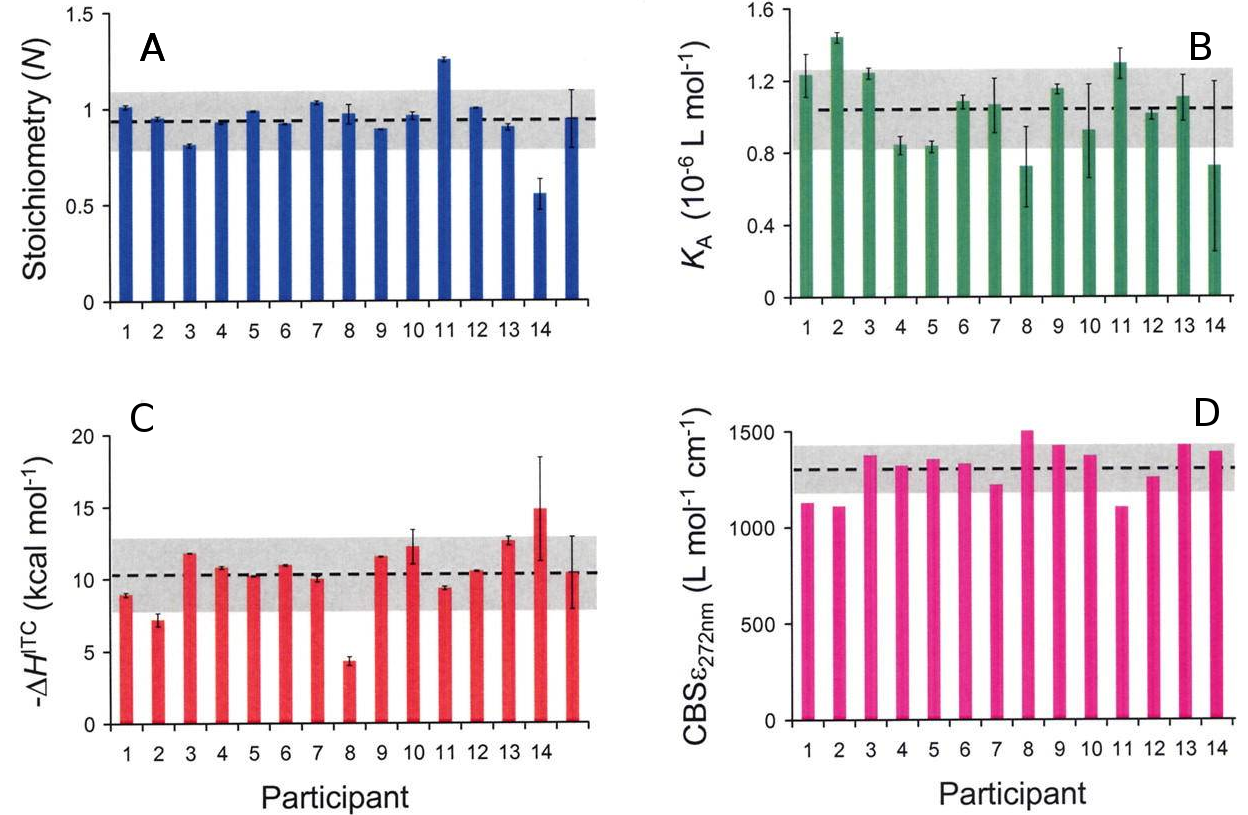
\includegraphics[width=\linewidth]{figures/cbs_ca_II.PNG}	
	\end{tikzfigure}

}

 % First column - second block
\block{Fitting baselines using Gaussian process regression}{
\begin{tikzfigure}[Since we integrate over peaks, we need reliable estimates of our baseline.]
 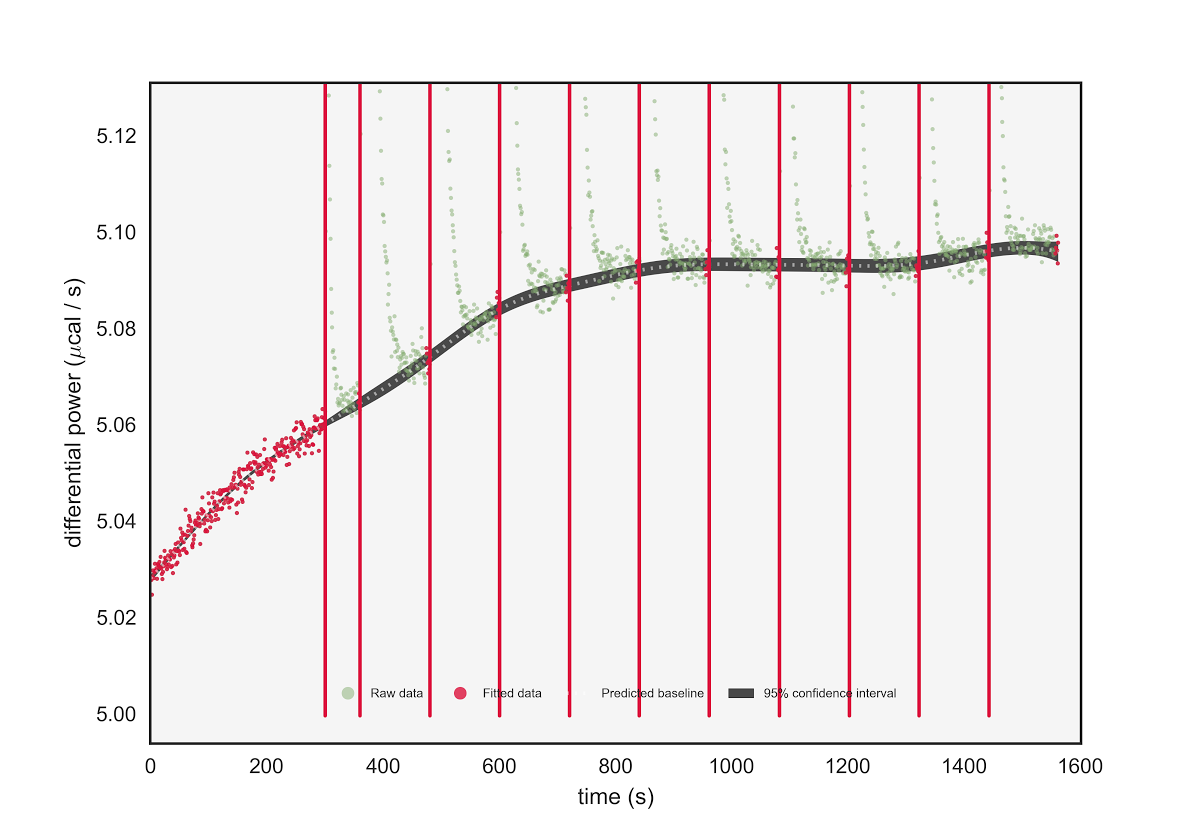
\includegraphics[width=\linewidth]{figures/baseline.png}
\end{tikzfigure}


}

 % First column - third block
\block{Sample Block 4}{T\\E\\S\\T}

 % SECOND column
\column{0.33}
 %Second column with first block's top edge aligned with with previous column's top.

 % Second column - first block
\block{A Bayesian approach to experimental analysis}{
\begin{tikzfigure}[\small In an ITC experiment, we inject from a syringe into a sample cell several times, measuring a differential power, and then integrating over that to obtain the heat of the injection, $q_n^\mathrm{obs}$.]
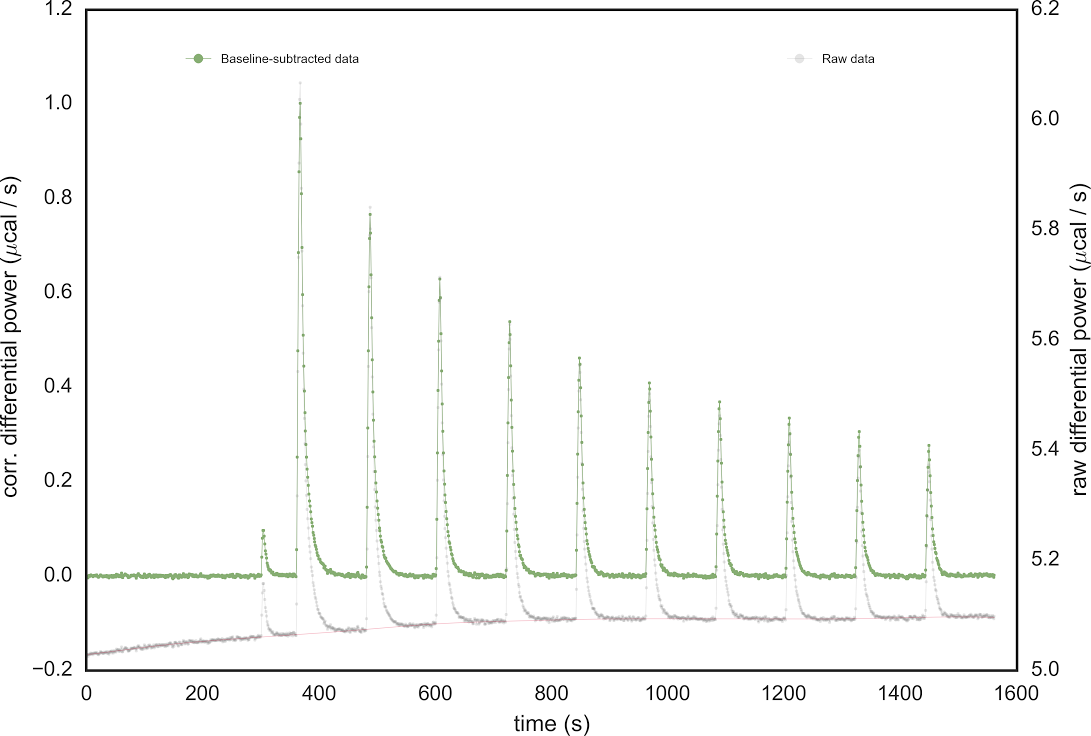
\includegraphics[width=\linewidth]{figures/itcexp.png}	
\end{tikzfigure}
According to the central limit theorem (CLT), we can model the integrated heats as being samples from a normal distribution $\mathcal{N}$,
\begin{align}
q_n^\mathrm{obs} \sim \mathcal{N}(q_n^\mathrm{true}, \sigma^2) \quad ,
\end{align}
with the true heats $q_n^\mathrm{true}$ as a mean, with a variance of $\sigma^2$. 
}

% Third column
\column{0.33}

\block{From likelihood to posterior density}{
Using Bayes rule, we can obtain a posterior distribution $\mathcal{P}\left(\theta | \mathcal{D} \right)$
\begin{align}
	\mathcal{P}\left(\theta | \mathcal{D} \right) \propto  \mathcal{P}(\mathcal{D} | \theta) \mathcal{P}\left(\theta\right) \quad .
\end{align}
Here, $\mathcal{P}\left(\theta\right)$ is a prior density of our parameters:
\begin{align}
	\theta   =  \left\{ \Delta G_\mathrm{bind}, \Delta H_\mathrm{bind}, \Delta H_0, [\mathrm{X_{syr}}], [\mathrm{M_{cell}}], \sigma \right\} \quad,
\end{align}
for which the distributions can be defined using prior knowledge about errors made by instrumentation.


}

\block[]{Markov chain Monte Carlo gives us probabilities for all our parameters}{
  \begin{tikzfigure}[An example distribution sampled for the syringe concentration.]
   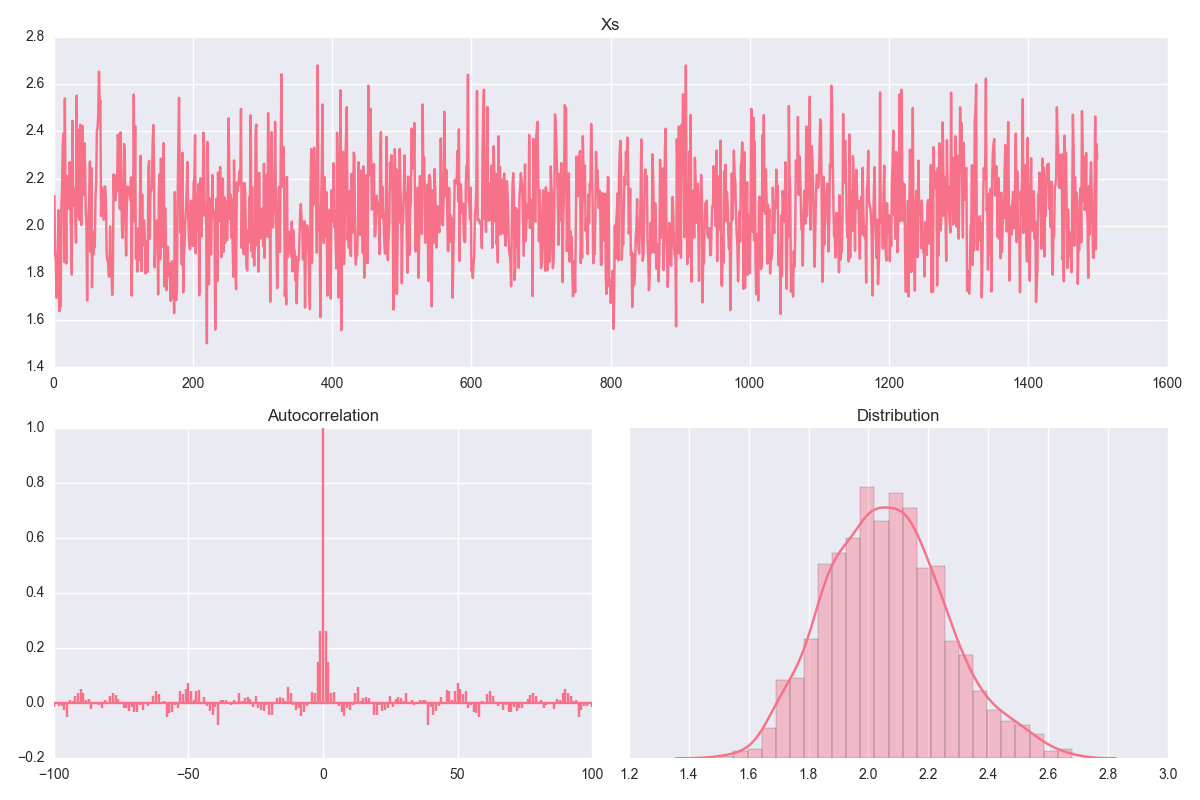
\includegraphics[width=\linewidth]{figures/sampling.png}
  \end{tikzfigure}

}


 % Second column - third block
\block{}{Block with no title}

 % Second column - A collection of blocks in subcolumn environment.
\begin{subcolumns}
    \subcolumn{0.27} \block{1}{First block.} \block{2}{Second block}
    \subcolumn{0.4} \block{Sub-columns}{Sample subblocks\\Second subcolumn}
    \subcolumn{0.33} \block{4}{Fourth} \block{}{Final Subcolumn block}
\end{subcolumns}


 % Bottomblock
\block{Conclusions}{ here is some text
}
\end{columns}
\block[titleleft, titleoffsetx=2em, titleoffsety=1em, bodyoffsetx=2em,%
 bodyoffsety=-2cm, roundedcorners=10, linewidth=0mm, titlewidthscale=0.7,%
 bodywidthscale=0.9, bodyverticalshift=2cm, titleright]
{References}{    \printbibliography[heading=none]
}

\end{document}



\endinput
%%
%% End of file `tikzposter-template.tex'.
